\documentclass[11pt,letterpaper]{article}
% vim: nospell

\usepackage{fancyhdr} % fancy headers
\usepackage{geometry} % page geometry package
% \usepackage{sectsty}  % change the size of sections
\usepackage{amsmath} % equations in \align
% \usepackage{comment}
\usepackage{enumitem} % fancy enumerators
\usepackage[linesnumbered,lined,ruled,commentsnumbered,shortend]{algorithm2e} % pseudocode
\usepackage{hyperref} % hyperlinks
\usepackage{graphicx} % including images
\usepackage{fancyvrb} % sophisticated verbatim text
\usepackage[dvipsnames]{xcolor}   % pretty colours

%
% geometry
%
% \hoffset    = -0.5in
\voffset    = -0.25in
% \textwidth  = 7in
\textheight = 8.5in
\headheight = 26pt

%
% fancyhdr
%
\pagestyle{fancy}

%
% algorithm2e
%
\SetKwProg{Fn}{Function}{}{}

\SetKwRepeat{Do}{do}{while}

\SetKw{KwSpawn}{spawn}
\SetKw{KwSync}{sync}
\SetKwFor{ParallelFor}{parallel\_for}{do}{end}

%
% secsty
%
%\sectionfont{\fontsize{12}{15}\selectfont}

%
% fancyvrb
%
\RecustomVerbatimCommand{\VerbatimInput}{VerbatimInput}%
{fontsize=\footnotesize,
  %
  frame=lines, % top and bottom rule
  framesep=1em, % separation between frame and text
  rulecolor=\color{Gray},
  %
  % label=\fbox{\color{Black}data.txt},
  label=\fbox{\color{Black}},
  labelposition=topline
  % commentchar=# % ignore lines starting with commentchar
}


\rhead{CSE416A\\Final Project}
\chead{High-Performance Graph Clustering}
\lhead{Peter Olson\\p.olson 441666}

\begin{document}

\section{Introduction}

Throughout the semester, we've explored many different algorithms for
graph analysis, and graph clustering specifically.  However, most of the
implementations of these algorithms that we've employed throughout the
semester have been sequential implementations in imprecise, higher-level
languages.  From a hardware perspective, there was performance left on
the table, as most modern laptops sport dual or quad-core processors,
and desktops with six, eight, and even greater numbers of cores are
becoming increasingly common.

The goal of this project is to identify a model for parallel computation
that readily suits graph analysis algorithms and examine the performance
of different graph algorithms.  The performance of different algorithms
with and without in-memory graph compression is of specific interest for
this project, as the machine being used for benchmarking is running a
16-core 32-thread AMD 2950X with 32 GiB of DDR4 at 2666MHz.

Reimplementing the algorithms discussed below is of secondary interest,
and, when possible, the benchmarks are conducted with existing,
well-tested implementations of the given algorithms.

\section{Algorithmic Challenges}

Graph algorithms present a unique challenge in developing work-efficient
parallel implementation due to their agonizingly sequential structure.
The typical flow for a graph clustering algorithm is to first calculate
some observation on a graph, then cut the graph based on that
observation, until there exists no more optimal cuts to make.

The necessary sequential ordering of each cut means that there is a
strict upper limit on the amount of parallelism achievable. That is to
say that, rather than taking a parallel approach to the entire problem,
one must try to extract as much parallelism as possible between
performing cuts on the graph.

\subsection{Local Clustering}

An interesting subset of algorithms that I wound up doing most of my
testing and experiments with were local graph clustering algorithms. To
a computer engineer like myself, \emph{local} algorithms typically means
that they're written for a shared-memory computational model, rather
than distributed memory. However, in the context of graph analysis,
\emph{local} clustering refers to a family of clustering algorithms
that, rather than finding clusters for all points in the graph, simply
find a cluster around a single point.

Local clusters, namely thanks to their smaller sample set, are more
easily found in a highly-parallel fashion, because the only cut
performed comes at the end of the algorithm.  Their working set is also
a small fraction of the total size of the graph, which means that
investigating the cluster around specific points of interest can be done
much more quickly.

\subsection{Data Challenges}

One final, more subtle aspect that makes graph clustering a challenging
problem to parallelize is the inherent work-imbalance implicit in the
data set.  Because each node has different characteristics in a graph,
algorithms runtimes differ depending on which node they're run on.
While this characteristic is of negligible importance for sequential
graph algorithms, the work-imbalance across a data set makes decomposing
the problem much more challenging.

Because work does not necessarily map evenly over nodes, decomposition
becomes more challenging than simple segmenting a set of nodes into
equal-sized chunks for each parallel worker to process. The naive,
segmenting approach to parallel processing may be functional, in this
case, but it provides very poor guarantees for resource utilization and
computational span.  Though work is often correlated with the edges in a
set, clustering is a node-oriented computation, and thus dependent on
the work associated with each node.

\section{Ligra and Parallel Computation Models}

Ligra (\url{https://github.com/jshun/ligra}) is a parallel
graph-processing framework written in C++ which uses CilkPlus. Ligra's
model for parallelism is based on mapping computation over subsets of
the vertices in a graph, which one can think of as a moving frontier.
This `frontier-based' approach to parallelizing graph clustering, thanks
to the natural similarity to one step in a global clustering algorithm
to a single map operation. Ligra also offers a filtering model, wherein
the frontier is reduced by some metric, which is also well-suited to the
model of a graph clustering algorithm.

One very important part of Ligra's performance is the fact that it uses
CilkPlus, which is a work-stealing runtime system. In Cilk's parallel
model, parellism can be expressed as function calls that can execute in
parallel, points where the parallel function calls need to join, and
parallel for loops, where each iteration of the loop is processed in
parallel. Cilk's terminology for this model is \texttt{spawn}, 
\texttt{sync}, and \texttt{par\_for}.

Because Cilk is work-stealing, though, once a parallel worker runs out
of work that it can do on its own, the worker will attempt to randomly
steal work from other workers. Because a worker is either working or
attempting to steal, Cilk is able to guarantee real-world span that is
very close to optimal, even in cases where there is no readily apparent
way to decompose the work into equal amounts for each parallel worker.

\section{Algorithm Discussion}

Betweenness clustering (see Algorithm 1) is a great example of this
structural limitation for graph-clustering algorithms.

{\centering
\begin{minipage}{0.9\linewidth}
\begin{algorithm}[H]
	\caption{Betweenness-Based Clustering}

	% Set the variable \Names and display names
	% \SetKwData{P}{primary}
	% Set functions
	\SetKwFunction{stock}{gn\_betweenness\_clustering}
	\SetKwInOut{Input}{input}
	\SetKwInOut{Output}{output}

	\Input{A graph $G$ and a desired number of clusters $k$}
	\Output{A set of subgraphs}

	\Fn{\stock (G, k)}
	{
		\While{$number\_connected\_components(G) > k$}
		{
			\If{$size(G) = 0$}
			{break\;}
			$edge\_betweenness \gets edge\_betweenness\_centrality(G)$\;
			$remove\_edge(G, max(edge\_betweenness))$\;
		}
		\Return $connected\_components(G)$\;
	}
\end{algorithm}
\end{minipage}
}

Each edge-removal cut is dependent on the full completion of the
edge-betweenness computation that preceeds it, which means that the only
place to extrace parallelism in the algorithm is in that
edge-betweenness calculation.  

{\centering
\begin{minipage}{0.9\linewidth}
\begin{algorithm}[H]
	\caption{Recusive Modularity Maximization}

	% Set the variable \Names and display names
	% \SetKwData{P}{primary}
	% Set functions
	\SetKwFunction{stock}{mm\_clustering}
	\SetKwFunction{recursive}{mm\_recurse}
	\SetKwInOut{Input}{input}
	\SetKwInOut{Output}{output}

	\Input{A graph $G$ and a maximum number of clusters $k$}
	\Output{A set of subgraphs}

	\Fn{\recursive (G, k, $q_0$, q)}
	{
		$B \gets modularity\_matrix(G)$\;
		$u \gets power\_iteration(B)$\;
		\If{$k \leq 1$ or $q_0 > q$}
		{
			return G\;
		}
		$S_{left} \gets \{v | v \in G \cup u[v] \geq 0 \}$\;
		$S_{right} \gets \{v | v \in G \cup u[v] < 0 \}$\;
		$k \gets k - 1$\;
		\If{$k >= 1$}
		{
			\Return $\{S_{left}, S_{right}\}$\;
		}
		$left\_graphs \gets \recursive(S_{left}, k, q_0, modularity(G, S_{left}))$\;
		$k \gets k - len(left\_graphs)$\;
		\uIf{k == 0}
		{
			\Return $\{left\_graphs, S_{right}\}$\;
		}
		\Else
		{
			$right\_graphs \gets \recursive(S_{right}, k, q_0, modularity(G, S_{right}))$\;
			\Return $\{left\_graphs, right\_graphs\}$\;
		}
	}

	\Fn{\stock (G, k)}
	{
		\Return \recursive$(G, k, 0, 0)$\;
	}
\end{algorithm}
\end{minipage}
}

Modularity maximization (see Algorithm 2) is a more complex algorithim
that offers much more opportunities for parallel speedup in each cut
step, because each cut step removes significantly more edges from the
graph at once. Each recursive step of modularity maximization can be
computed independently, which is beneficial to the spacial locality of
each parallel unit of work.


PageRank-Nibble is a local clustering algorithm which is presented by J.
Shun et.  al. in \emph{Parallel Local Graph Clustering}. The pseudocode
is reproduced in Algorithm 3. PageRank-Nibble is, notably, only a
function to compute a vector of node-weight pairs. Shun et. al. propose
a parallelized sweep-cup algorithm to make the final pass over the
points and decide on the final cluster.

{\centering
\begin{minipage}{0.9\linewidth}
\begin{algorithm}[H]
	\caption{PageRank-Nibble}

	% Set the variable \Names and display names
	% \SetKwData{P}{primary}
	% Set functions
	\SetKwFunction{stock}{PR-Nibble}
	\SetKwFunction{Self}{UpdateSelf}
	\SetKwFunction{Neighbor}{UpdateNeighbor}
	\SetKwInOut{Input}{input}
	\SetKwInOut{Output}{output}

	\Input{A graph $G$, a seed vertex $v$, an error margin $\epsilon$, and
	a teleport probability $\alpha$}
	\Output{A set of subgraphs}

	$p \gets \{\}$\;
	$r \gets \{\}$\;
	$r' \gets \{\}$\;

	\Fn{\Neighbor (s, d)}
	{
		$r'[d] \gets r'[d] + (1-\alpha)r[s]/(2d(s))$\;
	}

	\Fn{\Self (v)}
	{
		$p[v] \gets p[v] + \alpha r[v]$\;
		$r'[v] \gets (1-\alpha)r[v]/2$\;
	}

	\Fn{\stock (G, k)}
	{
		$r \gets {(x, 1)}$\;
		$Frontier \gets \{x\}$\;
		\While{$Frontier > 0$}
		{
			$vertexMap(Frontier,\Self)$\;
			$edgeMap(G, Frontier,\Self)$\;
			$r \gets r'$\;
			$Frontier \gets \{v | v \in G \cap r[v] \geq d(v)\epsilon\}$\;
		}
		\Return p\;
	}
\end{algorithm}
\end{minipage}
}

\section{Discussion}

Unfortunately, despite the wonderful interface of Ligra, implementing
graph clustering algorithms in C/C++ is a bit of a nightmare. Both C and
C++ lack efficient semantics for working with and manipulating sets of
data points (similar to those found in higher-level languages, like
Python).  I didn't anticipate how difficult correctly implementing
either modularity-maximization clustering or PageRank-Nibble would be.
You can find my partial (very non-functional) attempts at
implementing them in \texttt{src/\{MM\_Clustering.C,PR-Nibble.C\}}.

The data taken below is from J. Shun's implementation of
PageRank-Nibble, which can be found in Ligra's \texttt{localAlg}
applications on GitHub.  I burned so much time trying to re-implement
these algorithms that I had very little time to analyze the data that I
collected. In addition to the graph comparing the performance of
compressed and uncompressed representations of the graph, I also have
data on the performance of PageRank-Nibble versus the traditional Nibble
algorithm, but I didn't have the time to analyze it before submitting
the report.

The data was run on the orkut network from SNAP
(\url{https://snap.stanford.edu/data/com-Orkut.html}).

I was, honestly, fairly surprised to see how little of
an impact in-memory compression made for the runtime of the clustering
algorithm. In the past, I had heard that graph analysis algorithms are
so memory-bandwidth intensive that in-memory compression could actually
accelerate the algorithm by alleviating some of the strain on the memory
interface. However, in this case, the compressed graphs are always
slightly worse than uncompressed graphs in both total runtime and
computational runtime.

Just as expected, PageRank-Nibble demonstrates excellent speedup when
scaling from one to 32 processor cores.

\begin{center}
	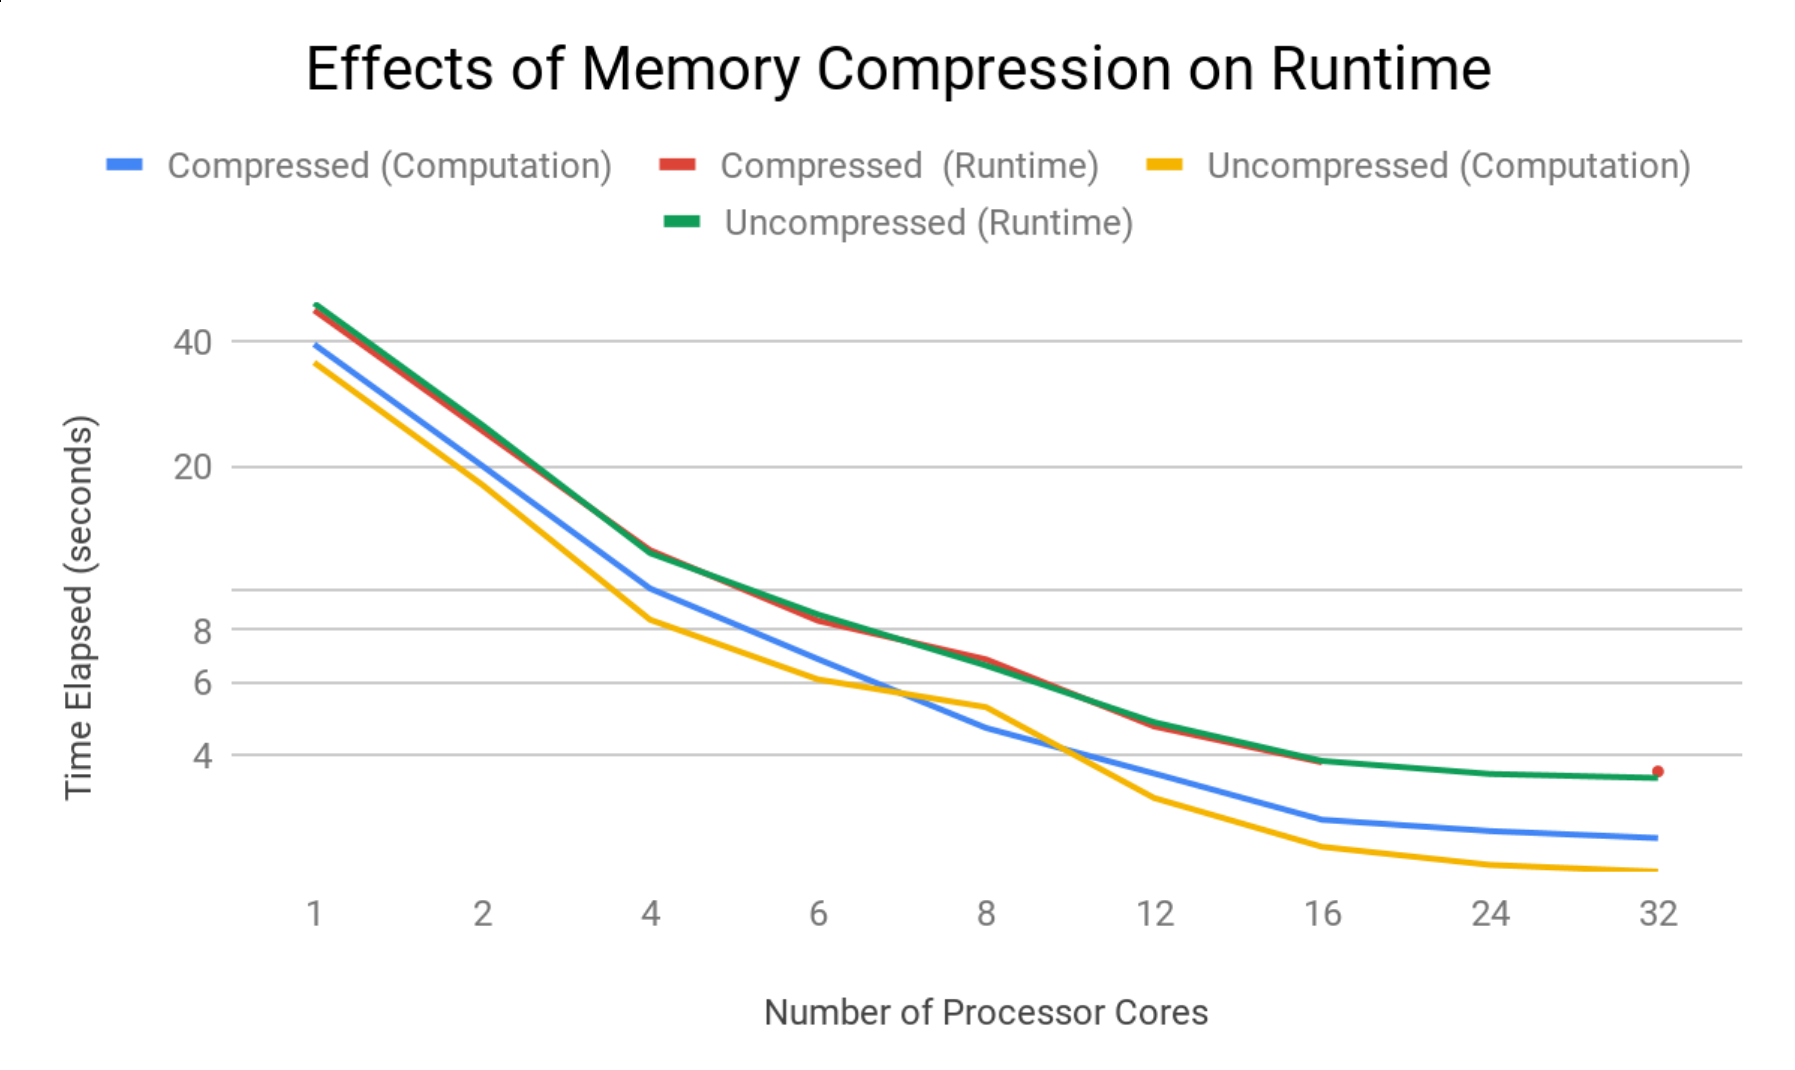
\includegraphics[width=0.75\linewidth]{../data/graph.png}
\end{center}


\section{Sources} $\ $

\url{https://people.eecs.berkeley.edu/~jrs/papers/partnotes.pdf}

\url{http://people.csail.mit.edu/jshun/local.pdf}

\url{https://github.com/jshun/ligra}

\url{https://www.cilkplus.org/}

\end{document}
